\documentclass[compress]{beamer}
\usepackage{ifthen,verbatim}

\title{Experiences with Alignment on the CAF \\ -- or -- \\ Validation of 1\_5\_4 Samples}
\author{Jim Pivarski, Alexei Safonov}
\institute{Texas A\&M University}
\date{24 August, 2007}

\newcommand{\isnote}{}
\xdefinecolor{lightyellow}{rgb}{1.,1.,0.25}
\xdefinecolor{darkblue}{rgb}{0.1,0.1,0.7}

%% Uncomment this to get annotations
%% \def\notes{\addtocounter{page}{-1}
%%            \renewcommand{\isnote}{*}
%% 	   \beamertemplateshadingbackground{lightyellow}{white}
%%            \begin{frame}
%%            \frametitle{Notes for the previous page (page \insertpagenumber)}
%%            \itemize}
%% \def\endnotes{\enditemize
%% 	      \end{frame}
%%               \beamertemplateshadingbackground{white}{white}
%%               \renewcommand{\isnote}{}}

%% Uncomment this to not get annotations
\def\notes{\comment}
\def\endnotes{\endcomment}

\setbeamertemplate{navigation symbols}{}
\setbeamertemplate{headline}{\includegraphics[height=1 cm]{../cmslogo} \hspace{0.1 cm} \includegraphics[height=1 cm]{../tamulogo} \hfill
\begin{minipage}{5.5 cm}
\vspace{-0.75 cm} \small
\begin{center}
\ifthenelse{\equal{\insertpagenumber}{1}}{}{\textcolor{blue}{\insertsection}}
\end{center}
\end{minipage} \hfill
\begin{minipage}{4.5 cm}
\vspace{-0.75 cm} \small
\begin{flushright}
\ifthenelse{\equal{\insertpagenumber}{1}}{}{Jim Pivarski \hspace{0.5 cm} \insertpagenumber\isnote/\pageref{numpages}}
\end{flushright}
\end{minipage}\mbox{\hspace{0.2 cm}}}

\begin{document}
\frame{\titlepage}

\begin{notes}
\item This is the annotated version of my talk.
\item If you want the version that I am presenting, download the one
labeled ``slides'' on Indico (or just ignore these yellow pages).
\item The annotated version is provided for extra detail and a written
record of comments that I intend to make orally.
\item Yellow notes refer to the content on the {\it previous} page.
\item All other slides are identical for the two versions.
\end{notes}

\begin{frame}
\frametitle{What I did}
\begin{itemize}\setlength{\itemsep}{0.5 cm}
\item Read events from DrellYan\_mumu\_40/CMSSW\_1\_5\_4-RelVal (ideal
and short-term (10 pb$^{-1}$ scenarios), turned them into AlCaRecoMu
format, and wrote to my personal CASTOR area

\item Ran a simple globalMuon alignment: inflated alignment parameter
errors for muon system to refit globalMuon tracks to tracker only,
then compared track $-$ hit residuals in the muon system

\item Both processes performed on the CAF

\item Conclusion: the samples look good, but I have intermittent
technical problems accessing the data
\end{itemize}
\end{frame}

\begin{frame}
\frametitle{Problem \#1 with file I/O}

(A) AlCaRecofication method that hardly ever worked:
\begin{itemize}
\item Select all files at once ({\tt vstring fileNames =
\{everything\ldots\}}) and split jobs with {\tt skipEvents = N*10000,
maxEvents = 10000}.

\item Most jobs were unresponsive for days, so I gave up on them

\item Perhaps this requires all files to be loaded in a cache
somewhere, which taxes resources
\end{itemize}

\vfill
(B) AlCaRecofication that works:
\begin{itemize}
\item One file per job

\item There's probably an optimum of 10 or 100 files, didn't explore
\end{itemize}

\vfill
Maybe this isn't a ``problem,'' maybe the system wasn't designed for method A.
\end{frame}

\begin{frame}[fragile]
\frametitle{Problem \#2 with file I/O}

About half of the files I created (with either method) can't be read back.

\scriptsize
\begin{verbatim}
[HIPAlignmentAlgorithm] constructed.
%MSG
%MSG-e FwkJob:  PoolSource:source{*ctor*} 22-Aug-2007 18:31:09 CEST pre-events
<FrameworkError ExitStatus="8002" Type="StdLibException" >
  Standard library exception caught in cmsRun
St9bad_alloc
</FrameworkError>

%MSG
%MSG-s StdLibException:  PoolSource:source{*ctor*} 22-Aug-2007 18:31:09 CEST  pre-events
Standard library exception caught in cmsRun
St9bad_alloc
\end{verbatim}

\vfill \normalsize
Standard library allocation error?  (No version mismatch)
\end{frame}

\begin{frame}
\frametitle{Data quality in two files that worked}

\begin{itemize}
\item 10,000 short-term scenario events (miscal and misalign) and 10,000 ideal events
\end{itemize}

Z peak in short-term scenario, using globalMuons fitted to the tracker: event generation is okay, tracker is okay

\begin{center}
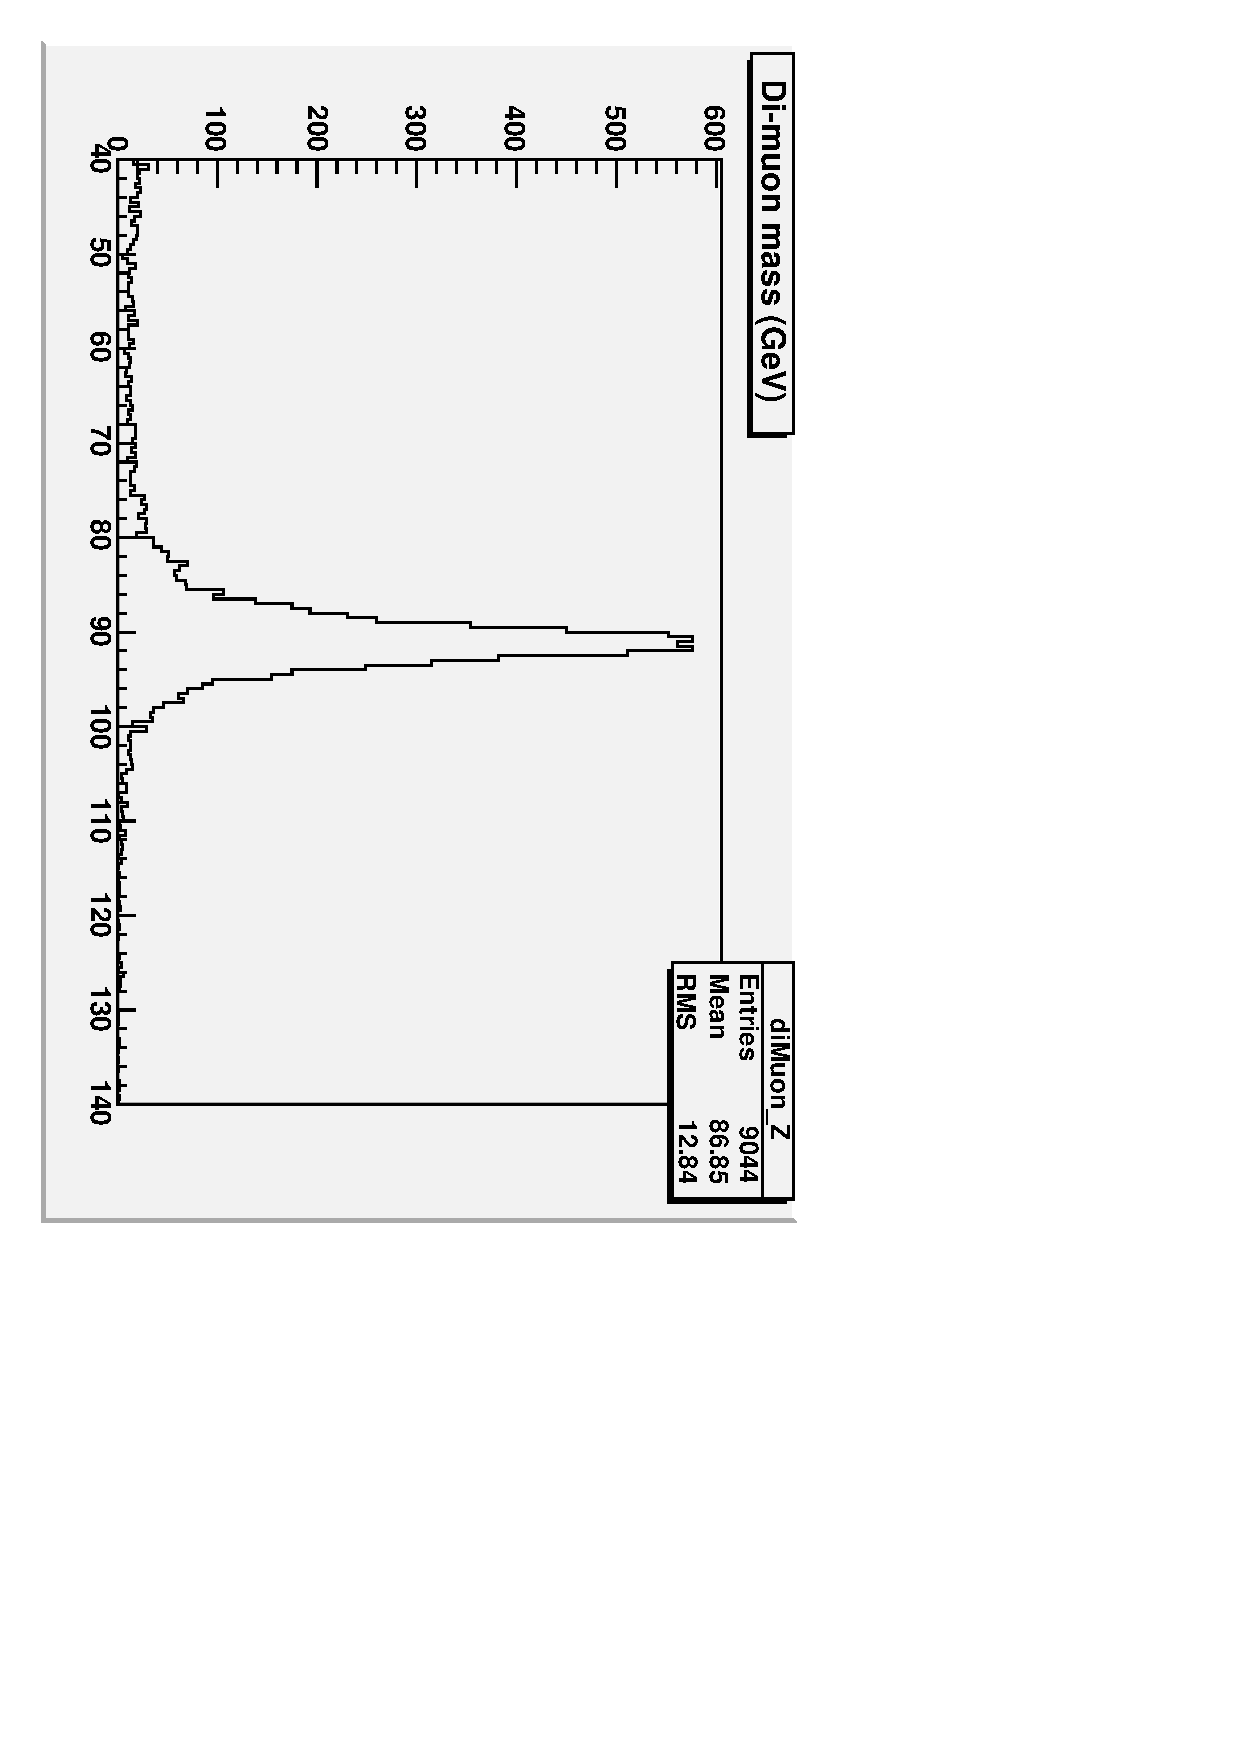
\includegraphics[height=0.7\linewidth, angle=90]{deweighted_short_zpeak.pdf}
\end{center}
\end{frame}

\begin{frame}
\frametitle{Residuals in the muon system}

\begin{itemize}
\item Again, tracks fitted to the tracker, extended to the muon system
\end{itemize}

\begin{center}
\begin{tabular}{p{0.45\linewidth} p{0.45\linewidth}}
\begin{minipage}{\linewidth}
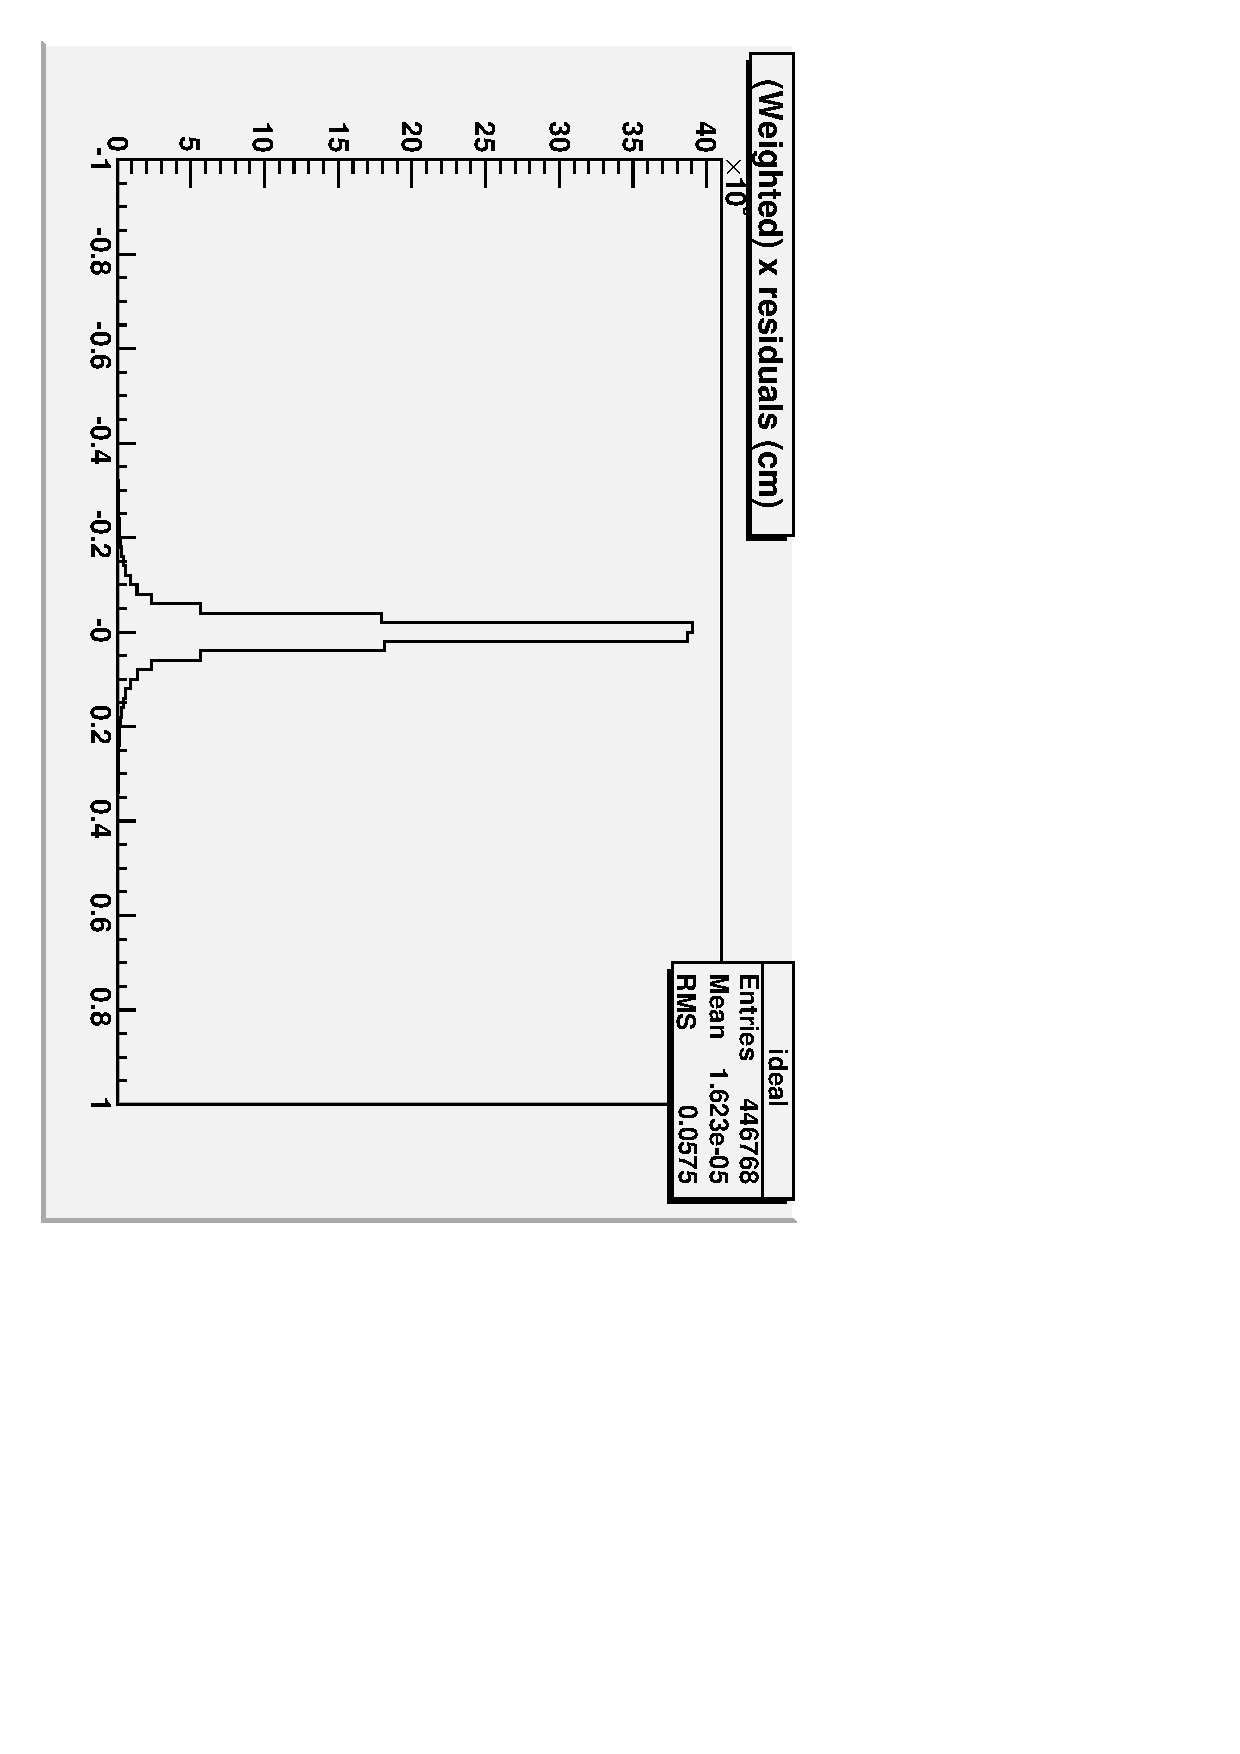
\includegraphics[height=\linewidth, angle=90]{deweight_outin_ideal.pdf}
\end{minipage} &
\begin{minipage}{\linewidth}
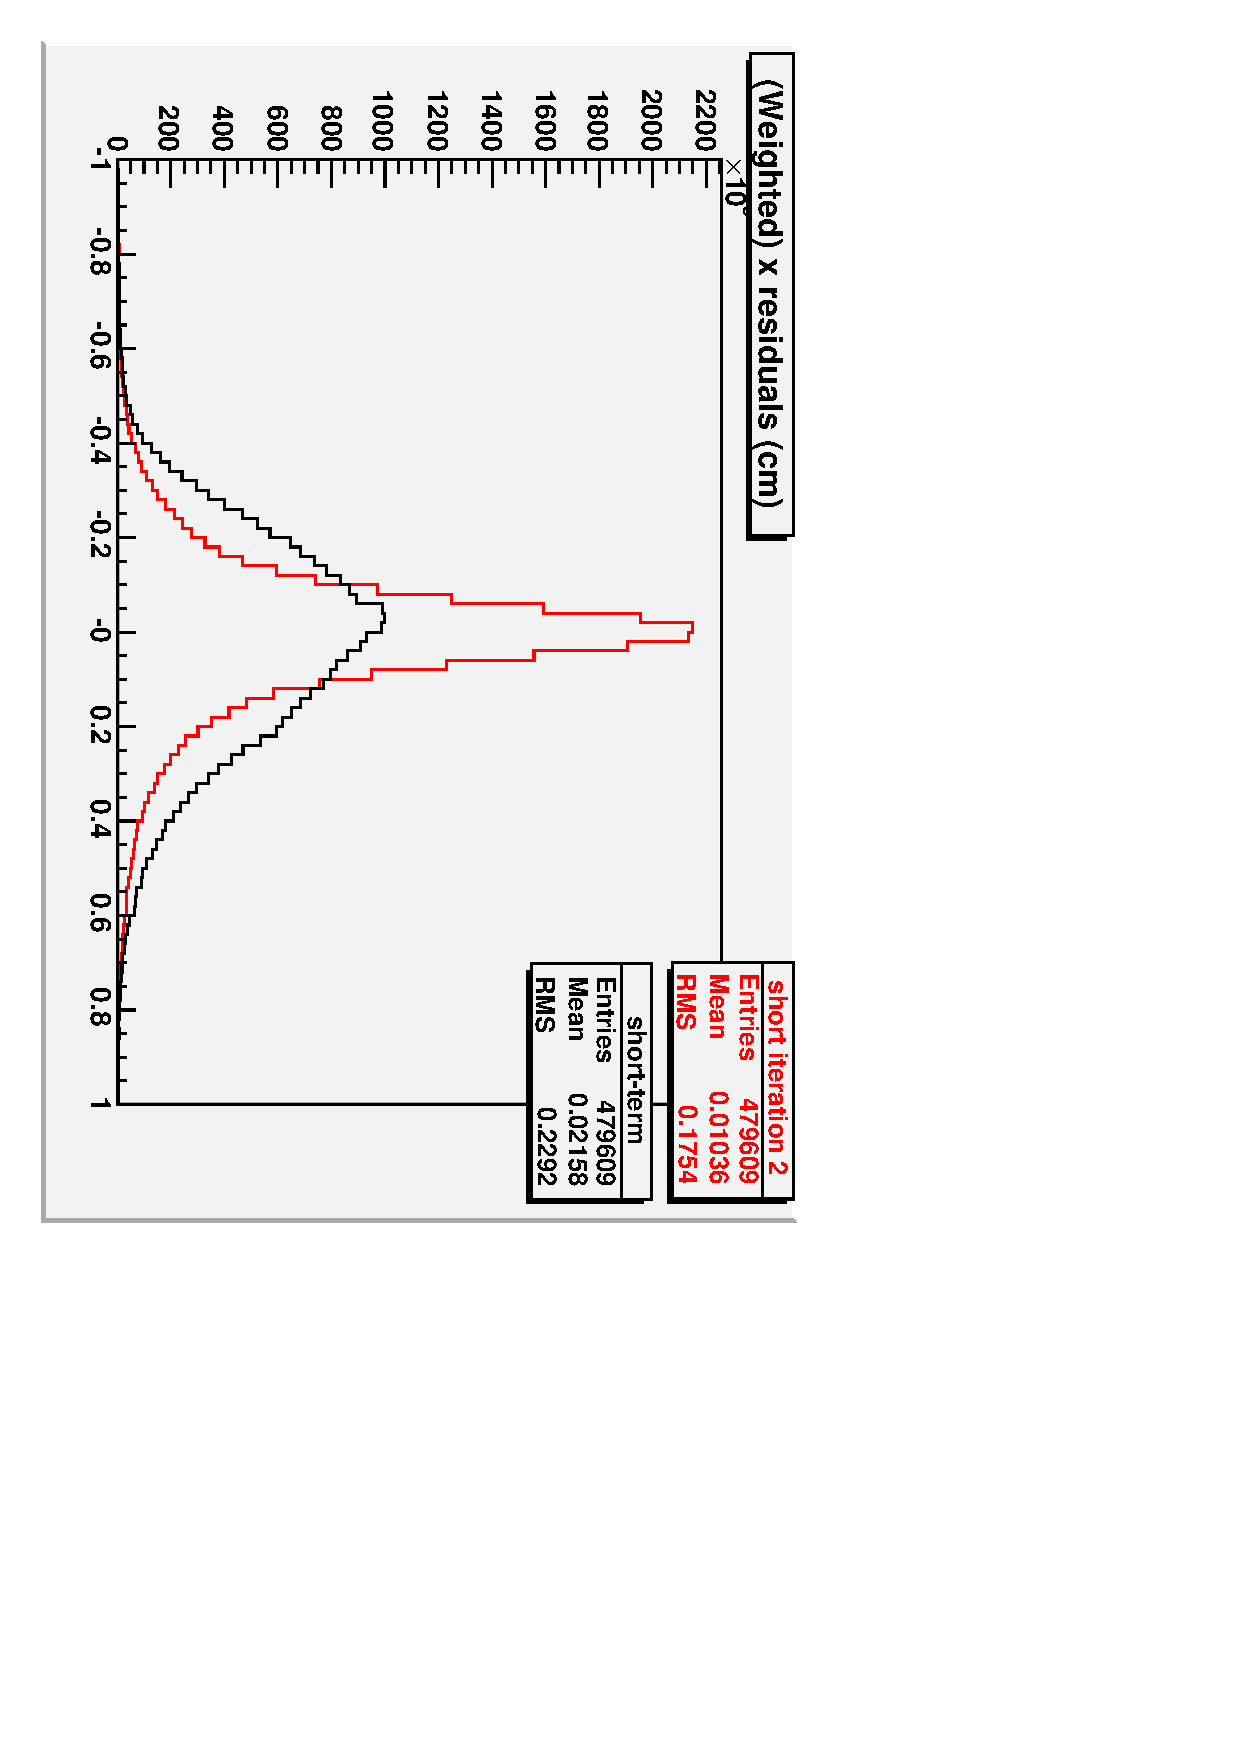
\includegraphics[height=\linewidth, angle=90]{deweight_outin_short.pdf}
\end{minipage} \\
\begin{minipage}{\linewidth}
\begin{center}
Ideal
\end{center}
\end{minipage} &
\begin{minipage}{\linewidth}
\begin{center}
Short-term
\end{center}
\end{minipage}
\end{tabular}
\end{center}

\vfill \textcolor{red}{Red} short-term is a quickie alignment: $x$ and
$\phi_z$ only, chamber-by-chamber, one iteration ($\sim$300/790 chambers aligned).

\vfill RMS from 2.3 mm $\to$ 1.8 mm, with ideal being 0.6 mm
\end{frame}

\begin{frame}
\frametitle{Typical single-chamber residuals distribution \#1}
\begin{center}
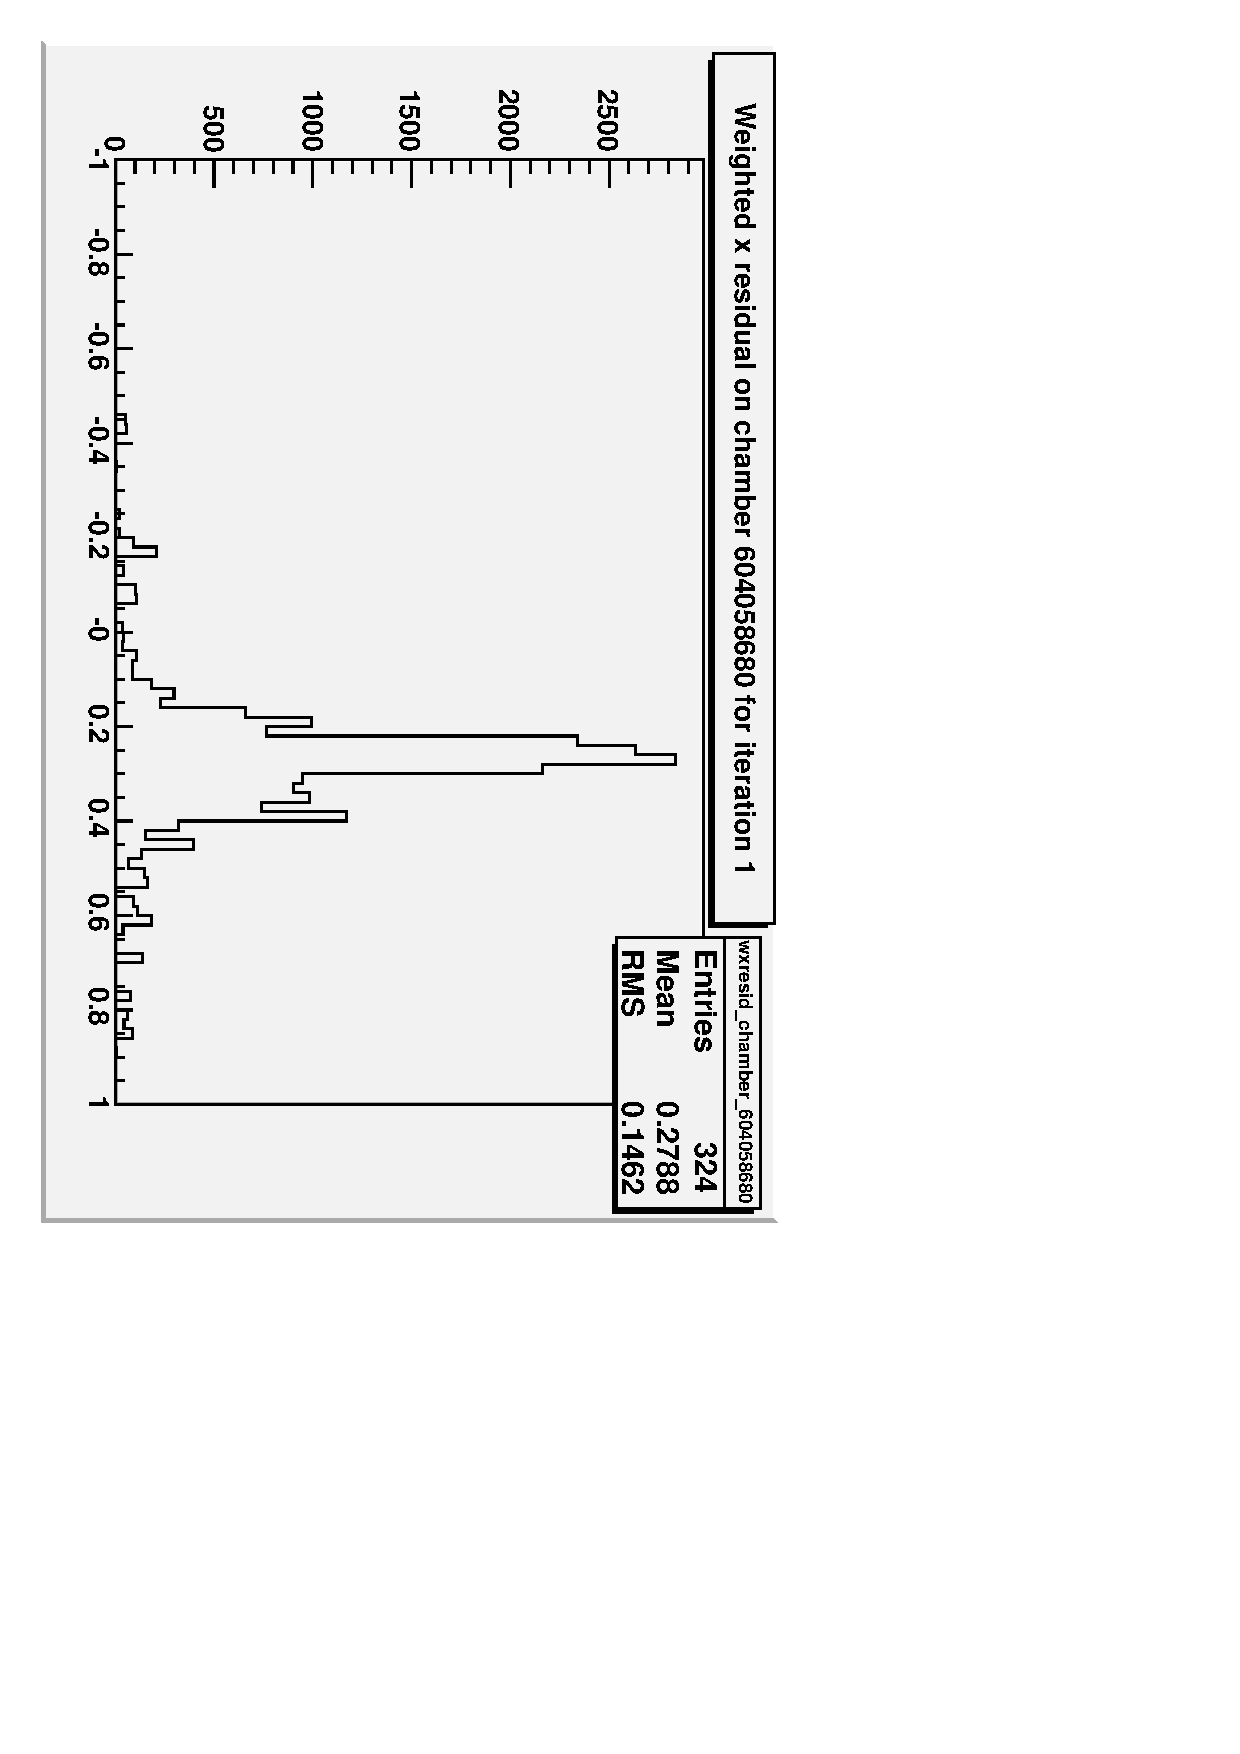
\includegraphics[height=0.7\linewidth, angle=90]{typical_short_deweight_outin.pdf}
\end{center}

\vfill
Cleanly misaligned
\end{frame}

\begin{frame}
\frametitle{Typical single-chamber residuals distribution \#2}
\begin{center}
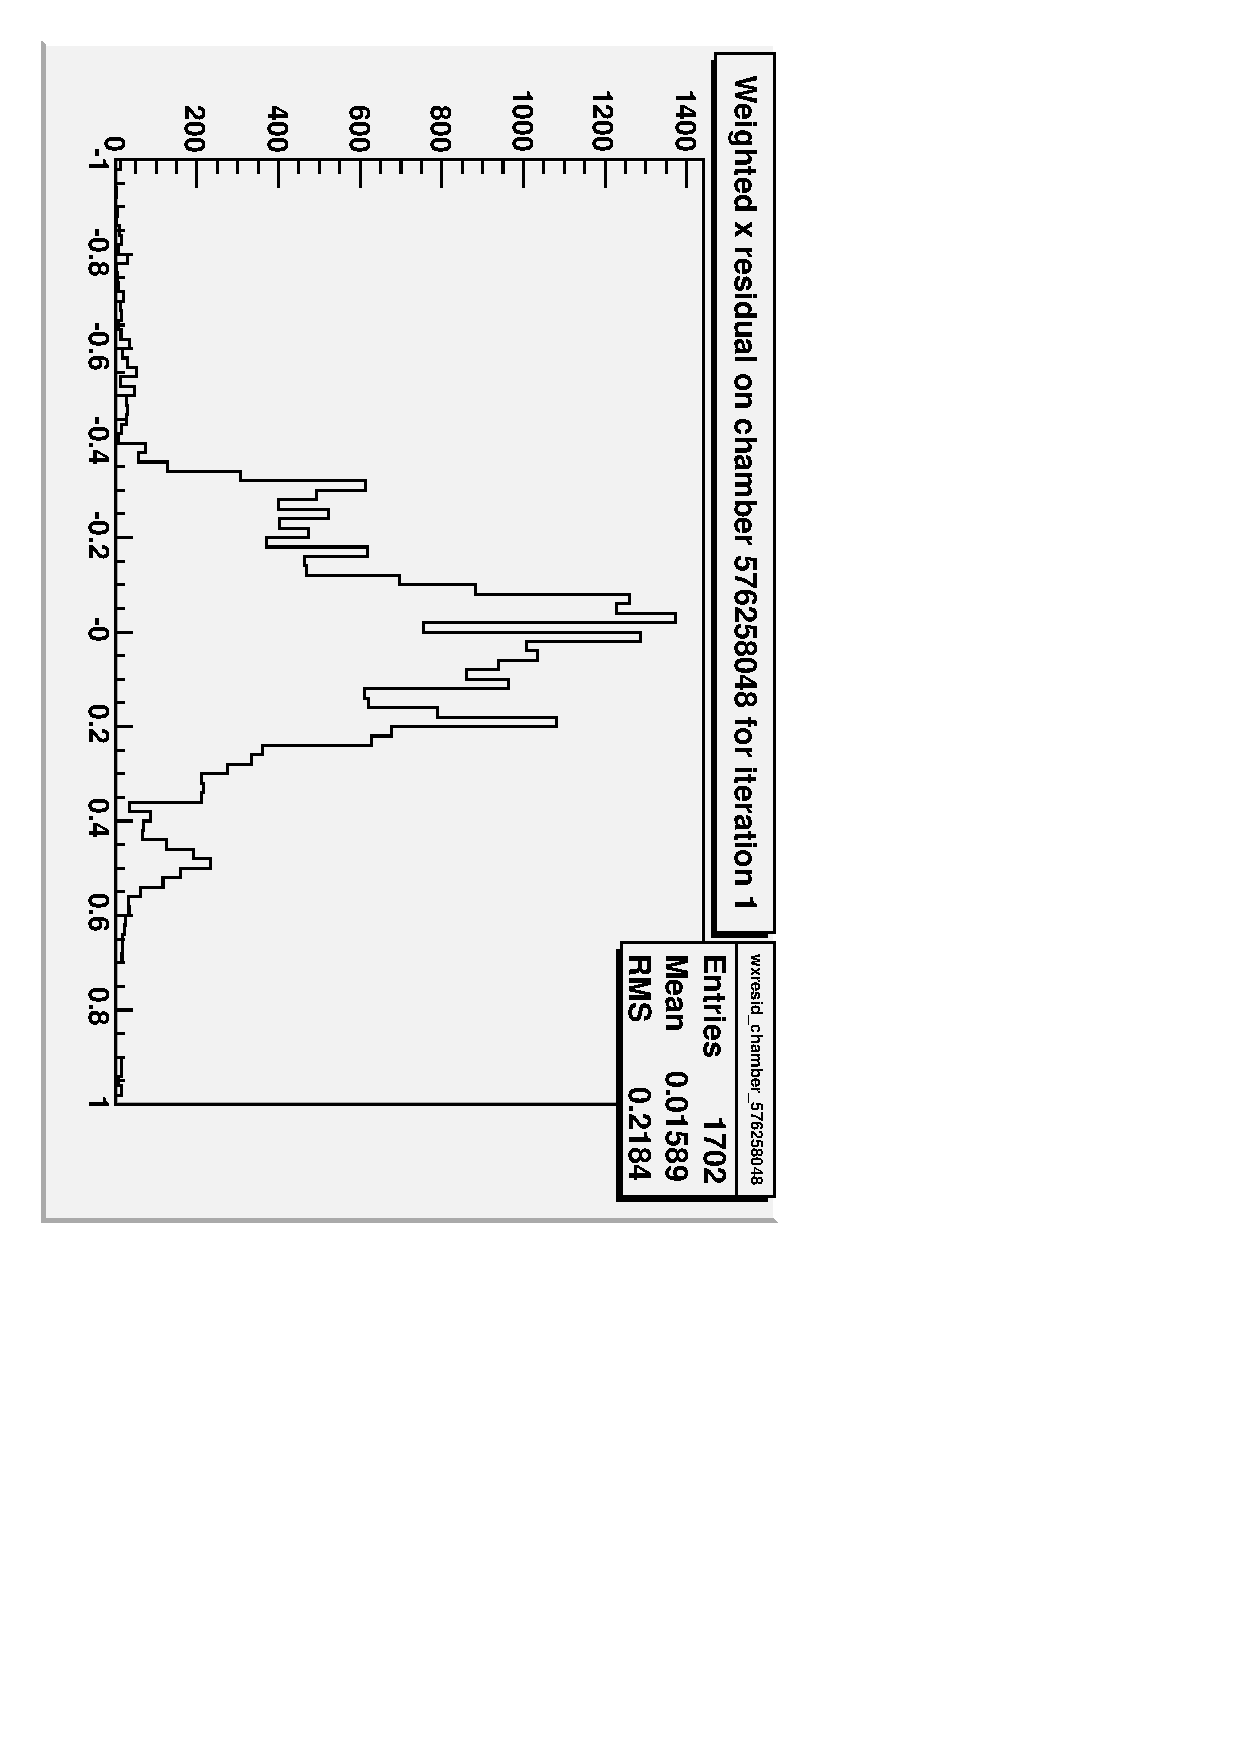
\includegraphics[height=0.7\linewidth, angle=90]{typical2_short_deweight_outin.pdf}
\end{center}

\vfill Internal structure.  Muon alignment short-term scenario does
not include internal (layer) misalignment.  Does calibration?
\end{frame}

\begin{frame}
\frametitle{Is this the right amount of misalignment?}

\begin{center}
\begin{tabular}{p{0.5\linewidth} p{0.5\linewidth}}
\begin{minipage}{\linewidth}
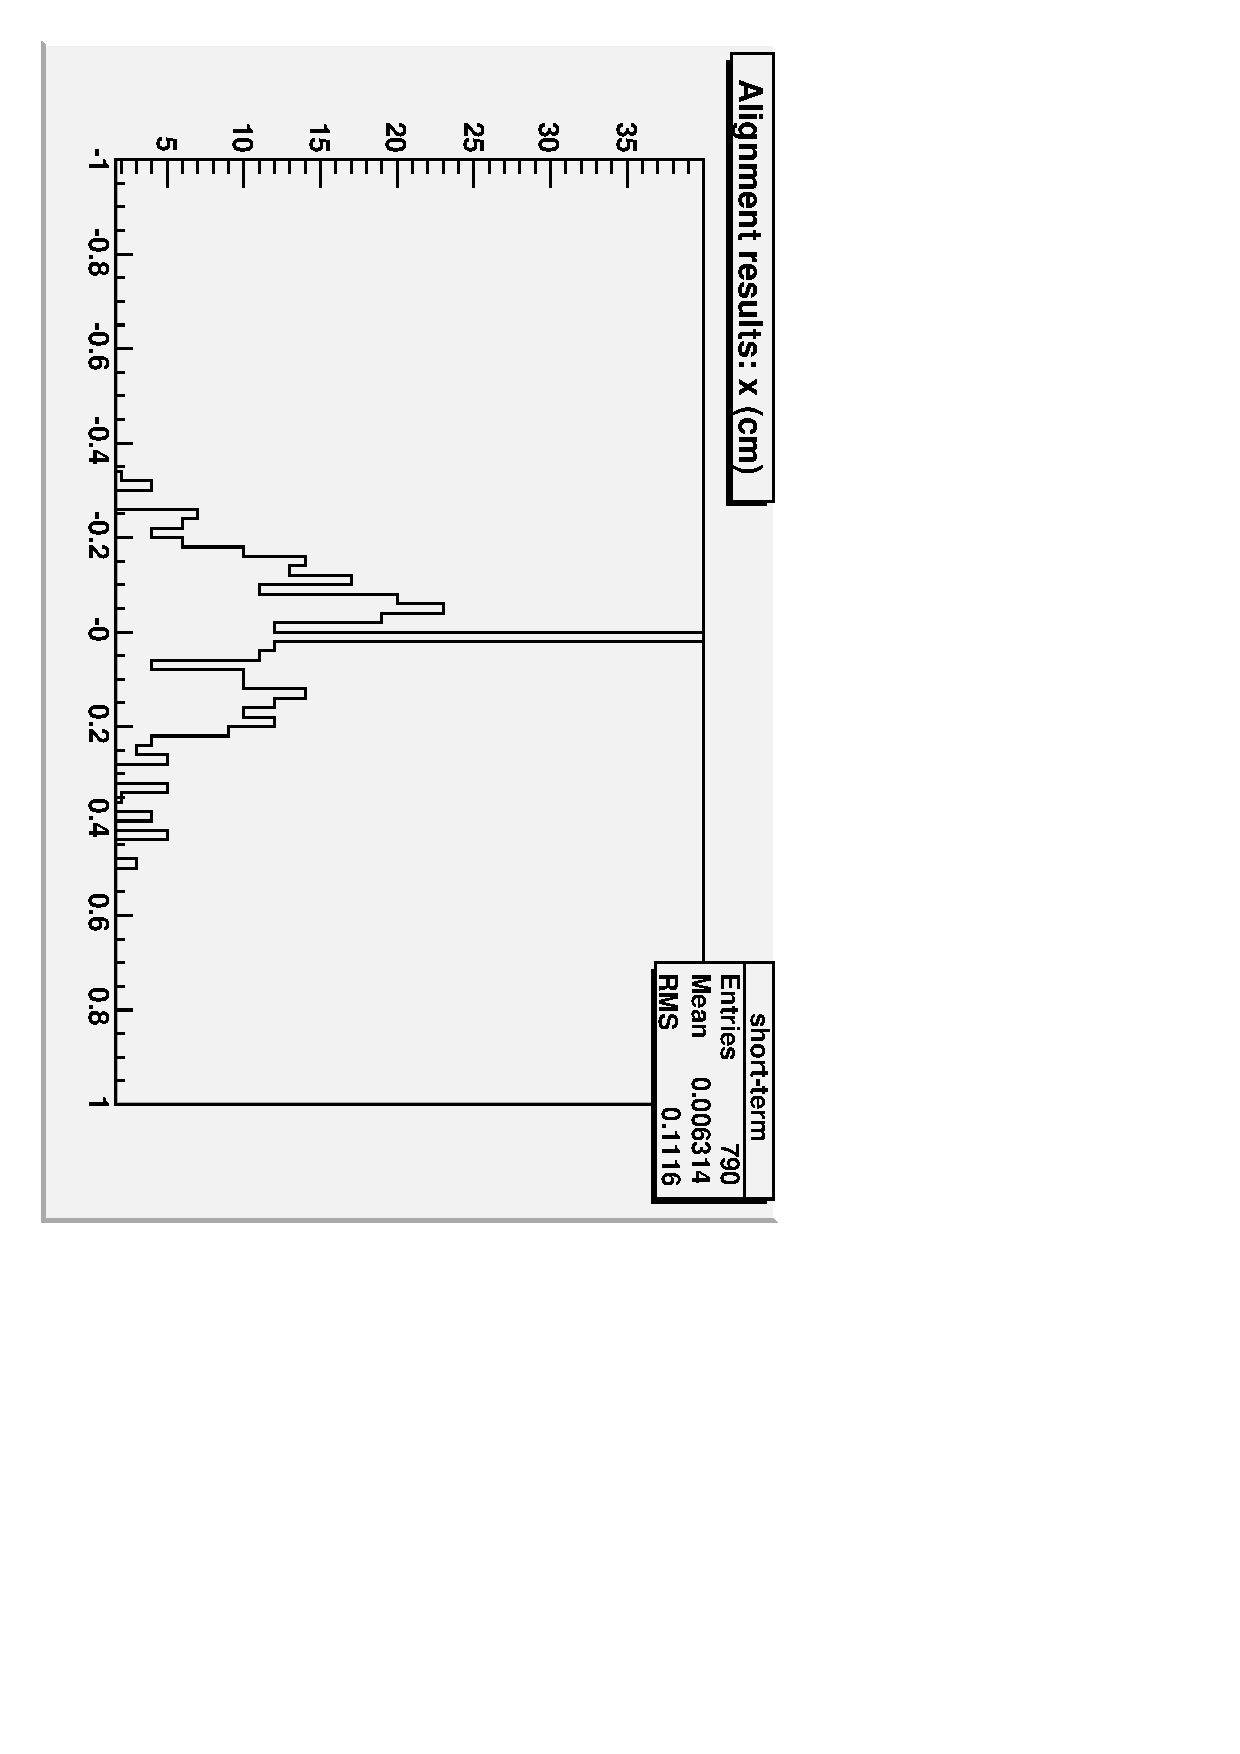
\includegraphics[height=\linewidth, angle=90]{alignment_results_x.pdf}
\end{minipage} &
\begin{minipage}{\linewidth}
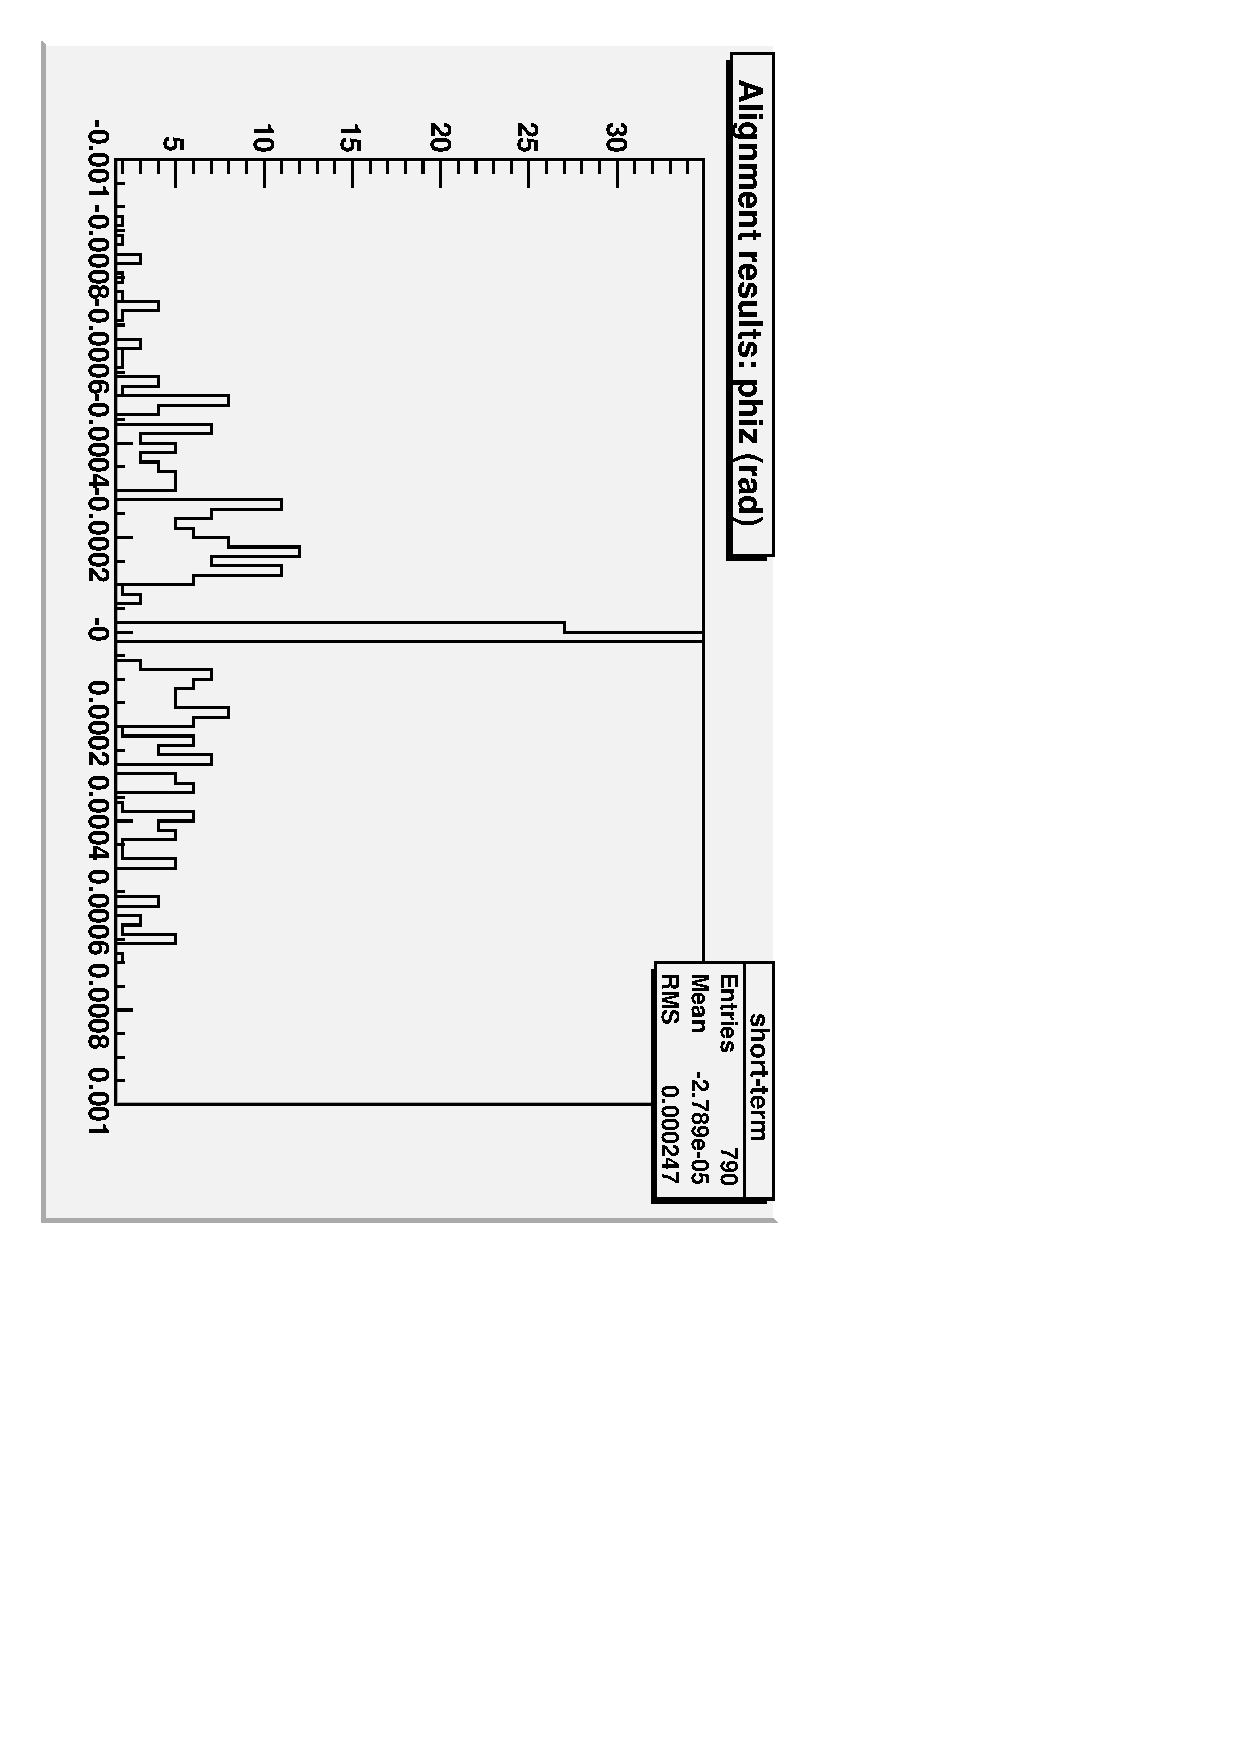
\includegraphics[height=\linewidth, angle=90]{alignment_results_phiz.pdf}
\end{minipage} \\
 & \\
\begin{minipage}{\linewidth}
Yes: $x$ misalignment dominated by wheel/disk, 0.2--0.25 cm
\end{minipage} &
\begin{minipage}{\linewidth}
Yes: $\phi_z$ both wheel/disk and chamber, 0.25 mrad
\end{minipage}
\end{tabular}
\end{center}

\vfill \vfill (Majority of chambers did not align because they didn't have the
minimum number of required hits)

\vfill \mbox{ }
\end{frame}

\begin{frame}
\frametitle{Conclusions}

\begin{itemize}\setlength{\itemsep}{0.75 cm}
\item The samples look fine!

\item AlCaRecofying will take some work, because of I/O problems.

\begin{itemize}\setlength{\itemsep}{0.5 cm}

\vspace{0.25 cm}
\item The one-file-per-job method successfully reads, but many of the
files it writes are broken.

\item There are over 2000 files!  It's easy enough to put 2000 jobs on
the CAF queue, but I couldn't test each of them for the ``Standard
library allocation'' error separately.

\item Any suggestions would be welcome!
\end{itemize}

\end{itemize}

\label{numpages}
\end{frame}

\end{document}
